%!TeX encoding=utf8

\section{Quantum Machine Learning}

\section{Stark Effect}

\subsection{Problems}
\begin{itemize}
        \item hyperfine structure negligible (normally when $\vec{E}$ is strong enough)
        \item perpendicular and transverse (formulas?)
        \item perturbation theory issue: states without $\vec{E}$ are square-integrable, with not (resonances of finite width, which have decay time, but for lower states its approximately stable), watch out for high $\vec{E}$
        \item in semiconductor enhance Stark-Effect because in the bigger band gap materials the holes and electrons are pulled in different directions, and not compensated by those in smaller band gap material
\end{itemize}

\subsection{Questions}
\begin{itemize}
    \item ion trap or superconductor?
    \item which atom are we looking at (degenerated, just lower states?)
    \item perturbation theory
    \item Runge-Lenz-Vector $\Rightarrow$ exactly solvable approximate model for an atom in strong oscillatory $\vec{E}$
\end{itemize}

\section{Quantum-confined Stark Effect (QCSE)}
\subsection{Problems}
\begin{itemize}
    \item $\vec{E_{ex}}$ absorption spectrum or emission spectrum of a quantum well
    \item electron states shift to lower energies, while the hole states shift to higher energies
        $\Rightarrow$ reduces the permitted light absorption or emission frequencies
    \item Holes and electrons pulled to different sides $\Rightarrow$ decreasing overlap integral $\Rightarrow$ reduces recombination efficiency
    \item Quantum Objects (Wells, Dots or Discs, for instance) emit and absorb light generally with higher energies than the band gap of the material, the QCSE may shift the energy to values lower than the gap.
    \item perturbation theory
    \item redshift for optical transition and decreases magnitude of absorption coefficient
    \item effect of excitons: $ h \nu > E_g - E_X $ with $E_X$ as energy of exciton (like hydrogen atom)
    \item $\vec{E}$ applied to bulk semiconductor, redshift also trough Franz-Keldysh effect, this one is limited by the absence of exciton as to strong $\vec{E}$ pull holes and electrons apart, this doesn't happen for QCSE as $\mathrm{e^-}$ are confined in quantum wells
    \item quantum wells behave as 2D $\Rightarrow$ enhance excitonic effects ($E_X$ 4 times larger than in 3D)

\end{itemize}

\section{Qiskit Pulse}

\subsection{Calibrating Pulse}

\begin{itemize}
    \item what are measurement\_map ?
    \item meas\_level=0 returns raw data (an array of complex values per shot), meas\_level=1 returns kerneled data (one complex value per shot), and meas\_level=2 returns classified data (a 0 or 1 bit per shot) $\Rightarrow$ what is measured?
    \item why is there some hard-coded 8 and 16? fft?
    \item What are the different channels, what are they for? (drive, acquire, measure)
    \item why is $\omega_{rabi,rough} + \omega_{detune}- \omega_{0}$ helping experimentally over $\omega_{rabi,rough} - \omega_{0}$ ?
    \item Why is Dynamical decoupling removing static noise?
\end{itemize}


\begin{figure}[H]
    \centering
    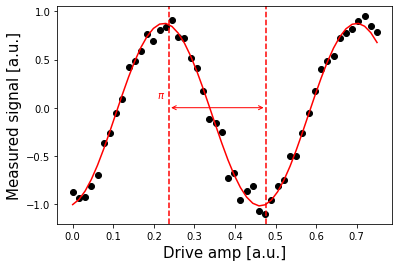
\includegraphics[width=0.7\textwidth]{IMAGE/rabi_osc.png}\\
    \caption{Normally rabi-oscillation are $P_g$ population in ground state over t, while $\vec{E}$ is a constant wave (constant amplitude), but here we have pulses.}
    \textsc{qiskit-textbook}, \emph{Calibrating Qubits Pulse} (2019)
    \label{fig:rabi}
\end{figure}


\begin{figure}[H]
    \centering
    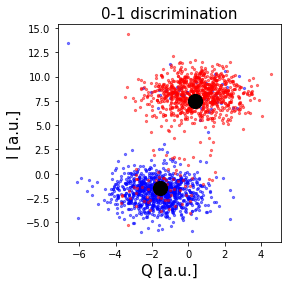
\includegraphics[width=0.7\textwidth]{IMAGE/excitation_ground_state.png}\\
    \caption{The blue cluster is $\ket{0}$ and red cluster is $\ket{1}$. But which physical quantity is measured (complex value of what?) }
    \textsc{qiskit-textbook}, \emph{Calibrating Qubits Pulse} (2019)
    \label{fig:ground}
\end{figure}


\begin{figure}[H]
    \centering
    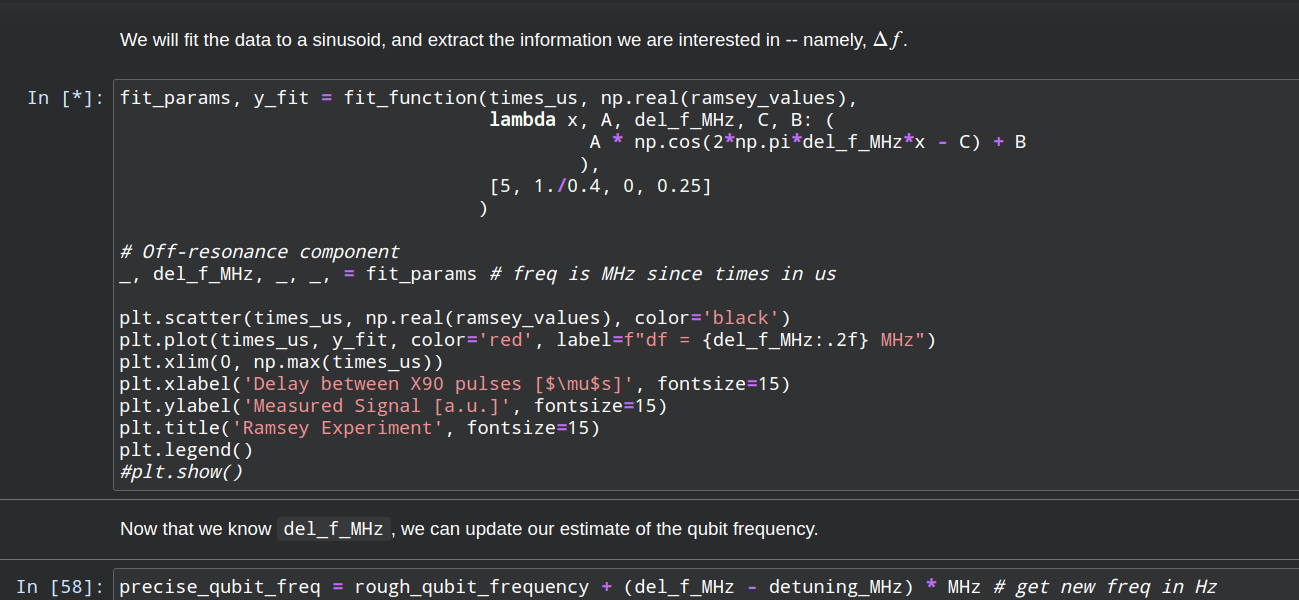
\includegraphics[width=0.7\textwidth]{IMAGE/ramsey_delta_f_missing_half.png}\\
    \caption{Probability for excited state is $P_{g} = \cos^{2} \left(\Delta t \cdot \frac{\left( \omega - \omega_{0}\right)}{2} \right)$ }
    \textsc{qiskit-textbook}, \emph{Calibrating Qubits Pulse} (2019)
    \label{fig:half}
\end{figure}


\subsection{Accessing Higher Energy States}

\begin{itemize}
    \item What does the following mean? The Pulse specification requires a single local oscillator frequency per schedule.
    \item The pulses to get to higher levels need to be shorter than the half time of the state? In state $\ket{1}$ the population is going down fast, so measuring the next energy jump is much harder. Where are the limits?
\end{itemize}

\begin{figure}[H]
    \centering
    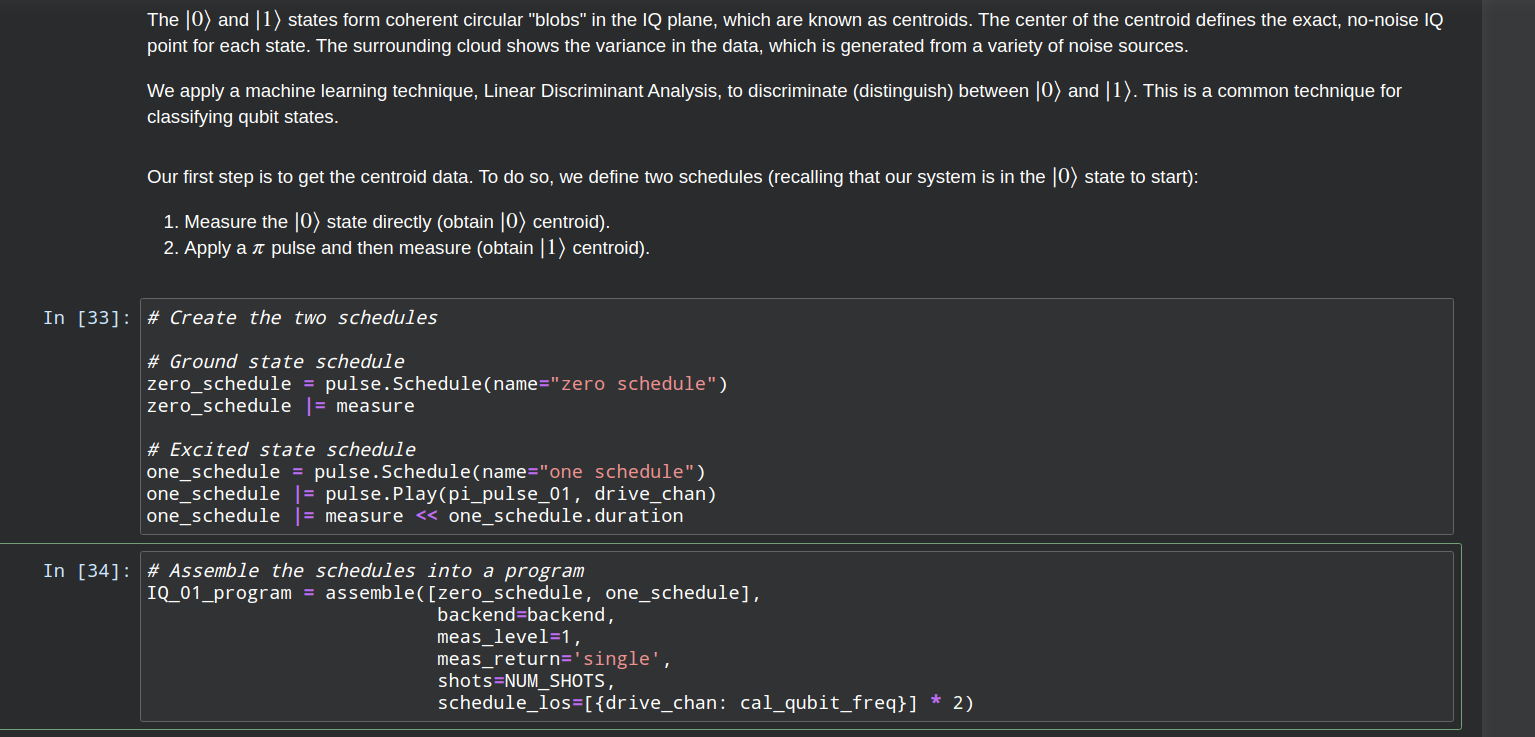
\includegraphics[width=0.7\textwidth]{IMAGE/6_2_why_single.png}\\
    \caption{Why is the $meas\_return$ single here and before always average?}
    \textsc{qiskit-textbook}, \emph{Accessing Higher Energy States} (2019)
    \label{fig:single}
\end{figure}


\begin{figure}[H]
    \centering
    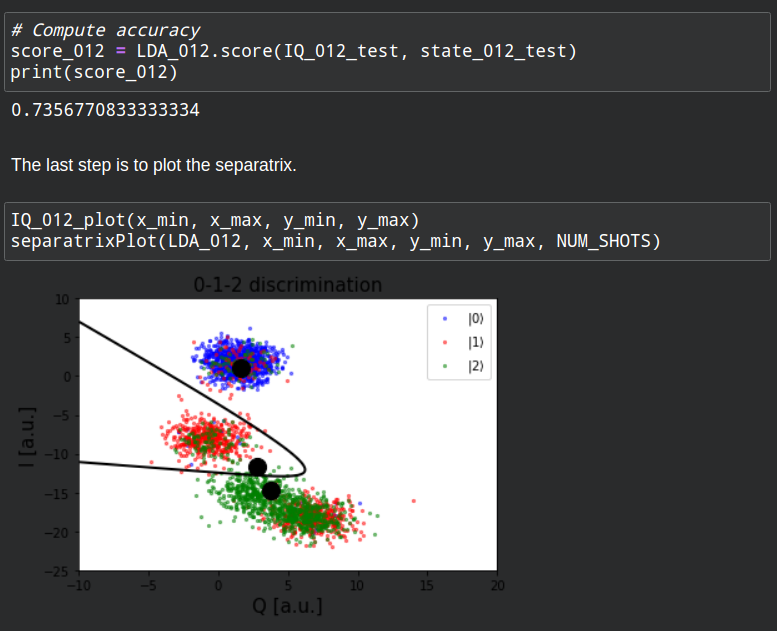
\includegraphics[width=0.7\textwidth]{IMAGE/6_2_bad_higher_level.png}\\
    \caption{What does the overlapping of the regions mean in terms of the system/calibration?}
    \textsc{qiskit-textbook}, \emph{Accessing Higher Energy States} (2019)
    \label{fig:single}
\end{figure}

\subsection{Circuit Quantum Electrodynamics}

\begin{itemize}
    \item regimes where the resonator acts as a perturbation to the qubit, perturbation theory (Schrieffer-Wolff transformation)
    \item Why is the drive part of the Hamiltonian block off-diagonal?
\end{itemize}


\begin{figure}[H]
    \centering
    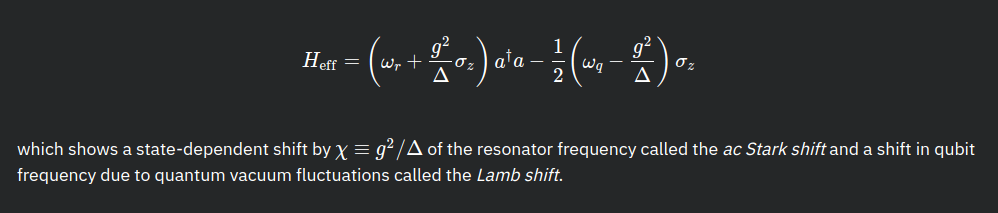
\includegraphics[width=0.7\textwidth]{IMAGE/6_4_james_cumming.png}\\
    \caption{James-Cumming Model}
    \textsc{qiskit-textbook}, \emph{Circuit Quantum Electrodynamics} (2019)
    \label{fig:james}
\end{figure}


\begin{figure}[H]
    \centering
    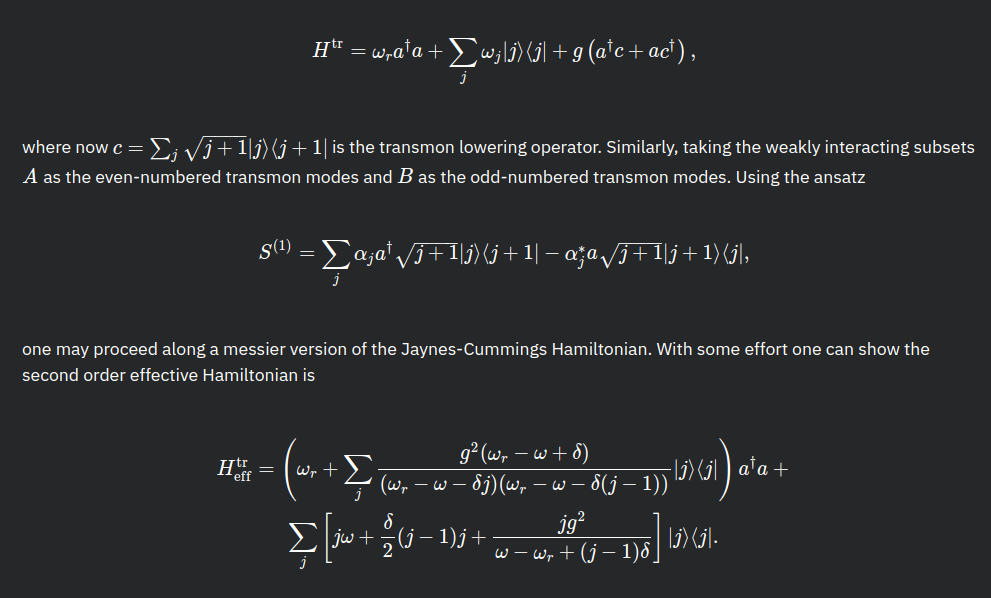
\includegraphics[width=0.7\textwidth]{IMAGE/6_4_transmon.png}\\
    \caption{Transmon qubit}
    \textsc{qiskit-textbook}, \emph{Circuit Quantum Electrodynamics} (2019)
    \label{fig:transmon}
\end{figure}
